\documentclass[10pt]{article}
\usepackage{itcep, stmaryrd, tikz, pgflibraryplotmarks, multicol}
\usepackage[margin=1in, nohead, pdftex]{geometry}
\usepackage{MnSymbol,wasysym}

\topmargin -0.2in
\pagestyle{empty}
\singlespacing
\let\oldhat\hat
\renewcommand{\vec}[1]{\mathbf{#1}}
\renewcommand{\hat}[1]{\oldhat{\mathbf{#1}}}

\definecolor{light-gray}{gray}{0.95}
\newcommand{\code}[1]{\colorbox{light-gray}{\texttt{#1}}}

\newcommand{\headerclass}{\code{<run>:\textbackslash the\textbackslash world} Machine Learning Camp}
\newcommand{\headersection}{Day 2: Exploring Data with Algorithms}
\newcommand{\headertitle}{Classification using (linear) Support Vector Machines}

\def\C{\mathbb{C}}
\def\R{\mathbb{R}}
\parindent 0ex
\begin{document}
%==================================================================================================================================================
\headerclass\xspace \hspace{\stretch{1}} \headersection\\
\begin{center}{ \large \textbf{\headertitle} }\end{center}
%==================================================================================================================================================





``Support vector machines'' are one way of classifying data observations. 
\begin{itemize}
\item Support: the support of a function is the set where the function isn't zero. Here it's really about where the function is positive and where it is negative.
\item Vector: an arrow that points to a point; a direction and a magnitude. A two-dimensional vector $\vec{x}$ is written $(x,y)$ or $(x_1, x_2)$, for instance. We will actually write \[\vec{x}_i = (x_{i1},x_{i2}).\]
\item Machine: it sounds cool! 
\end{itemize}
We'll start with \textit{linear} support vector machines, and in fact the simplest version: the ``maximal margin classifier''. The idea is that you pick a linear function like $f(\vec{x}) = 3x_1+2x_2-1$, and then you split your data into two classes using the line where that linear function equals zero. One of the classes should be on the side where $f(\vec{x}) > 0$ and the other class should be on the side where $f(\vec{x}) < 0$. (Yes, just two classes -- if you want to deal with more classes, you iterate this again and again.)
\bigskip
\begin{center}
Big idea: Pick linear functions to separate your groups
\end{center}
\bigskip

Fake data first:

Here is some fake data, designed to be nice. Can you draw a line to separate the two groups? (Can you draw more than one line?) Based on yesterday's activity, you know you can! But let's get more specific:
\begin{center}
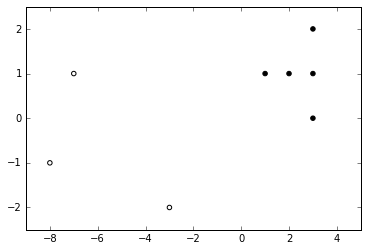
\includegraphics{TwoClusters.png}
\end{center}
\pagebreak
Compare the line you drew with the lines your neighbor drew. Some yes-no questions:
\begin{itemize}
\item[$\square$] If I removed the white point at (-8,-1), would you change your separating line?
\item[$\square$] If I removed the black point at (3,2), would you change your separating line?
\item[$\square$] If I removed the white point at (-7,1), would you change your separating line?
\item[$\square$] If I removed the black point at (3,0), would you change your separating line?
\end{itemize}
Talk with your neighbor -- do you agree?
\vspace{1in}
	
Given your discussion, which points do you think matter the most?

\vspace{1in}
The points that matter the most are the ones that give us the \textit{support vectors}.
\bigskip

Going back to the picture with the fake data, write down the equation of your line in $y=mx+b$ format:
\vspace{.75in}
Now transform it to write a function $f(x_1,x_2)$:
\begin{itemize}
\item change your $x$ to $x_1$
\item change your $y$ to $x_2$
\item move everything to the right-hand side
\item write \[f(x_1,x_2 ) = \underline{\hspace{2in}}\]
\end{itemize}

Plug in a few points to your new equation: if you plug in coordinates for white dots, do you get positive or negative numbers? If you plug in coordinates for black dots, do you get positive or negative numbers?
\vfill

If all the white dots give you outputs with the same sign from $f(x_1,x_2)$, and all the black dots give you outputs with the opposite sign, you have made your first \textit{separating hyperplane}.
\pagebreak

\begin{center}
\bf{The Support Vector Machine Algorithm in 2 dimensions}
\end{center}


How do we mathematically decide where the line between two groups should go? This is an \textit{optimization} problem. ``Optimal'' means ``best,'' measured in a specific mathematical way.

The people who invented support vector machines (SVM) decided that they wanted the widest possible ``street'' between the two groups of data. This is called the margin. I want to use a ``street'' analogy because you want a lane on each side of your separating line!

\begin{itemize}
\item This is a supervised learning problem, so you need data separated into two classes, labeled by $1$ and $-1$.
\item  You want to find the margin M (the ``width of the lanes in the street'') that is \textit{maximal}, as big as possible. Remember the ``street'' can contain no data. 
\item Here are the constraints for your data in two dimensions:
\begin{itemize}
\item You have points $\vec{x}_1, \ldots, \vec{x}_n$ in your training data. For instance, $\vec{x}_1 = (x_{11}, x_{12})$ and $\vec{x}_2 = (x_{21}, x_{22})$ and $\vec{x}_3 = (x_{31}, x_{32})$. 
\item Each point $\vec{x}_i$ has a label $y_i$, which is $1$ or $-1$ to reflect which class it's in.
\item You want to find weights $\beta_1$ and $\beta_2$ so that \[\beta_1^2 +\beta_2^2=1\] and \[y_i (\beta_0 + \beta_1 x_{i1} + \beta_2 x_{i2}) \geq M.\]
\end{itemize}
\end{itemize}

This optimization is not that hard if you are in multivariable calculus \smiley{} but if you are in algebra, trig, or single-variable calculus, this is hard. We'll talk through it.

\end{document}
